\DontNumberThisInToc
\DontFrameThisInToc
\Annex{Publications \label{annex:p}}
\begin{quote}
``The important thing in science is not so much to obtain new facts as to discover new ways of thinking about them'' (William Lawrence Bragg).
\end{quote}
%\ChapterNoNumberCitation{}{The important thing in science is not so much to obtain new facts as to discover new ways of thinking about them.}{William Lawrence Bragg}{10cm}
Ces travaux de thèse ont donné lieu aux publications suivantes: \\

\begin{itemize}
\item[$\bullet$]Chapitre de livre\\
\begin{itemize}
\item Taouali W., Rougier N. P., Alexandre F (2012).``Visual Target Selection Emerges from a Bio-inspired Network Topology'', Studies in Computational Intelligence, pages 317--330.\\
\end{itemize}
\item[$\bullet$] Revue\\
\begin{itemize}
\item Taouali W., Vieville T., Rougier N. P., Alexandre F (2011). ``No clock to rule them all '',  Journal of Physiology- Paris 105,1-3  83-90.\\
\end{itemize}
\item[$\bullet$]Conférences internationales avec comité de lecture\\
\begin{itemize}
\item Taouali W., Rougier N. P., Alexandre F (2010).`` Saccades generation : from the visual input to the superior colliculus'', dans International Conference on Neural Computation ICNC 2010 (Espagne).\\
\item Taouali W., Alexandre F., Hutt A., Rougier N. P (2009). ``Asynchronous Evaluation as an Efficient and Natural Way to Compute Neural Networks'', dans 7th International Conference of Numerical Analysis and Applied Mathematics – ICNAAM 2009 1168, pp. 554-558 (Grèce).\\
\end{itemize}
\item[$\bullet$] Conférences françaises\\
\begin{itemize}
\item  Taouali W., Viéville T., Rougier N., Alexandre F (2010). ``On Asynchronous Dynamic Neural Field Computation'', dans la Cinquième conférence plénière française de Neurosciences Computationnelles,
"Neurocomp'10".\\
\end{itemize}
\end{itemize}

Une revue et un article sont en cours de préparation. Le texte de la revue et du chapitre du livre publiés est dans la suite.\\


\section{No clock to rule them all}
\begin{center}
Wahiba Taouali, Thierry Vi\'eville, Nicolas Rougier et Fr\'ed\'eric Alexandre\\
Journal of Physiology Paris, 105,13  83-90.
\end{center}
\paragraph{abstract}
\textit{The hallmark of most artificial neural networks is their intrinsic parallelism
where each unit is evaluated concurrently to other units in a distributed way,
thus using {\em asynchronous} mechanisms.  However, this notion of asynchronous
computation is polymorphic and far from being obvious, as asserted by the
huge and somehow contradictory literature on this topic. Facing up the
related pragmatic issues, the goal of this article is twofold.  On
one hand, it precisely clarifies basic key notions related to asynchronous
distributed computations. On the other hand, a few practically usable methods
and quantitative bounds are made explicit.}


\subsection{Introduction}

%%  - Pourquoi aynchroniser : distribué + bio
%%     -- Do you think seriously your model is parallel and/or distributed ?
%%     -- One CPU to rule them all !
%%     -- Anyway, Nature is event-driven...
%%     -- Asynchronous computing for the dummies
%%  - Asynchrone pour les nuls
%% - What is the paper about:
%%  1. General framework
%%     - DNF (system)
%%     - Asynchronous definitions 
%%       -> au niveau general (or not ?)
%%       -> Specific case of DNF
%% General problematique (issues)
%%  2. before asynchronicity: discretization steps 
%%       => Space discretization (A priori fixed) 
%%       => Time  discretization (Euler & friends) Th 
%%       => Value discretization (Robert versus Mitra) Wa
%%  3. How to ensure convergence et calcul guaranty (at the very least -> Mitra) Wa
%%        (compared to synchronous computations)
%%         continuous value mitra
%%  4. Implementation: deds (discrete event dynamic system) Th


Brain is mostly event driven ! When a spike is sent along an axon, its processing is taken into account at the level of the dendrite (and later integrated in the soma), when arriving at the synaptic cleft. This triggers a complex chain of bio-chemical processings allowing the signal to be processed via the synapse and to be sent further along the dendrite, etc. There is consequently no need of any kind of central clock (or centralized signal) to coordinate such processing. This is truly distributed and asynchronous. And these properties are enforced anytime over the entire network (a.k.a. the brain). However, this does not prevent some synchronization to happen between neurons as it has been reported in a number of works, but this occurs only on the basis of local interactions without the need of any kind of central clock nor supervisor. If we now turn to the artificial neural networks paradigm, we realize that this asynchronicity property is hardly enforced in any model. Most numerical methods used to simulate the underlying differential evolution equations require an implicit central clock. Even the most complex and elaborated spiking neuron models are doomed with such considerations if they do not rely on explicit event-driven simulations\footnote{See e.g. \url{http://mvaspike.gforge.inria.fr/} for such implementation}. This is the case for synchronous computations, in which a central mechanism updates each unit (e.g. neuron model) at the same clock-time but less obvious is the fact that this is also the case for some asynchronous paradigms, in which, for instance, a central mechanism randomly draws without replacement the units to sample at a given regular clock time, in order to simulate asynchronous computation. The knowledge of which unit has been sampled or not must be centralized. More generally, usual strategies require a complete information about each part of the current state in order to deliver from a centralized locus the signal of the next step. Furthermore, this implies the random sampling events to occur at very regular times. It is thus implicitly assumed that the time is global to the whole system. Computation is distributed, but the computation time and clock remain centralized.

What are the consequences ? At the computational level, this means that if we are using a multi-processor architecture, processors that finish their task early have to wait, doing nothing, until others finish. The more synchronization points are set, the more performance degrades.  At the system dynamics level, such regular updates may induce spurious synchronization mechanisms.  At the biological modeling level, we must assume the existence of a global ``universal'' clock which is a reasonable approximation for small dynamical systems, but less obvious when considering several cortical maps in interactions with complex connection delays.

The goal of this article is thus to consider literature in relevant domains, namely cellular automata \cite{Fates:2005,Fates:2008,Garcia:2006,Barret:1999} and parallel computations \cite{Bertsekas:1991,Bertsekas:1997}, and to make the link with computational neuroscience. More specifically, we will introduce the dynamic neural fields theory that offer a very general computing framework for the modeling of cortical phenomena and since this theory is continuous in both space, time and values, we will pay special attention at the discretization procedure since we aim at using results from the discrete event systems specification to simulate discrete time systems and approximate, as closely as desired, differential equation systems. At this stage, we do not aim at giving a complete state-of-the-art on asynchronous models, but rather to show how a general construct, called here {\em fully asynchronous paradigm}, provides a constructive answer to asynchronous computation, especially in the particular case of artificial neural networks.

%% Thus, we briefly present in section~\ref{models} some computational models dealing with asynchrony aspects in discrete and continuous dynamic systems. Then, we focus in section~\ref{euler} on the bias induced by the discretization of continuous dynamic systems, allowing us to explain the foundation of well-defined asynchronous computation regarding dynamic neural fields, in section~\ref{mitra}.  Finally, we propose, in section~\ref{deds}, to use an event-driven paradigm, as an adequate framework to simulate an intrinsically asynchronous system, before concluding this work.

%% The DEVS formalism \cite{Zeigler:2000} provides a way of expressing discrete event models and a basis for an open distributed simulation of dynamic environments in which ``events`` occur. It also supports hierarchical modular construction, such as microscopic neurons, mescoscopic columns, etc. Using DEVS abstractions to capture the spiking nature features of biological neurons that were not represented in conventional artificial neural networks, started with Pioneer works of \cite{watts:1994, vahie:1996}, exploiting these capabilities to perform intelligent control tasks.

%% - What is the paper about:
%%  1. General framework
%%     - DNF (system)
%%     - Asynchronous definitions 
%%       -> au niveau general (or not ?)
%%       -> Specific case of DNF
%% General problematique (issues)
%%  2. before asynchronicity: discretization steps 
%%       => Space discretization (A priori fixed) 
%%       => Time  discretization (Euler & friends) Th 
%%       => Value discretization (Robert versus Mitra) Wa
%%  3. How to ensure convergence et calcul guaranty (at the very least -> Mitra) Wa
%%        (compared to synchronous computations)
%%         continuous value mitra
%%  4. Implementation: deds (discrete event dynamic system) Th


%% Since it is rather counter-intuitive to rely implicitly on such a centralized scheme, we would like to study to which extent we can remove this central clock assumption and implement a really decentralized (asynchronous) computation.

%%  This has been already studied in the case of cellular automaton \cite{Fates:2005,Fates:2008,Garcia:2006,Barret:1999} and parallel computations \cite{Bertsekas+Tsitsiklis91,Bertsekas+TsitsiklisBook97}

%% In this context, asynchronous mechanism at the mesoscopic level may represent:
%%  \\ - biological delays related to the cortical map topography, with three facets: 
%%         fixed delay related to known connection length, 
%%         dynamic delays related to on-going processing or transmission, random delays related to uncertainty or lack of knowledge about the two previous mechanisms;
%%  \\ - local computation effects such as adaptive asynchrony, i.e. the fact that a unit adapts its state with parsimony: 
%%         the more its value is stable, the less its change has to be output rapidly;
%%  \\ - mesoscopic events such as activity synchronization, rhythms, or sudden activity change.

%% As soon as such semantics is targeted, there is no place for a central mechanism to decide ``a-priori'' which unit is going to update its state, 
%% whereas each unit has to calculate on its own, both what is its next value and when its next value is going to be updated. 

\subsection{General framework}

\subsubsection{Dynamic Neural Fields}
Let us target generalized neural fields with delayed connection strength that are {\em tissue level models that describe the spatio-temporal evolution of coarse grained variables such as temporal synchronization or firing rate activity in populations of neurons} as explained by \cite{Coombes:2006}. Such neural fields were primarily introduced by \cite{Wilson:1973} and \cite{Amari:1977} and are generic enough to give account on a great number of models from the computational neuroscience community. We will consider a single {\em network} made of several {\em units} with {\em spatial connections} between them. The evolution of the activity $V$ of such a network is described by the following differential equation, which may write:
%%
\begin{align}
  \label{eq:DNF-continuous}
  & \frac{\partial V(\mathbf{x},t)}{\partial t} =
  -\frac{1}{\tau(\mathbf{x})} \, V(\mathbf{x},t) + h(\mathbf{x}, t) + s(\mathbf{x}, t)  \notag \\ 
  &+ \int_{\cal M} d \mathbf{y} \, \int_0^{+\infty} \, \hspace{-1em} d \eta \; W(\mathbf{x}, \mathbf{y}, \eta) \, \sigma_{\mathbf{y}}\left(V(\mathbf{y}, t - \eta)\right) 
\end{align}
%%
where $\mathbf{x}$ denotes a location onto the manifold $M$, $t$ is time, $V(\mathbf{x}, t)$ denotes the membrane potential of a neural population at point $\mathbf{x}$ and time $t$, ${\tau}$ is the temporal decay of synapses, i.e., represents a {\em leak}, $\eta$ is the transmission delay, $W$ is the (spatio-temporal) synaptic function, $s(\mathbf{x},t)$ is the input received at position $\mathbf{x}$ and $h$ is the mean neuron threshold.

In this framework, $\sigma_{\mathbf{y}}()$ is a smooth sigmoid function that relates the unit state to the mean firing rate. As an extension of this {\em analog} input/output non-linearity, steep sigmoid profiles can also be introduced in order to encounter for mesoscopic events triggered by some unit state. Furthermore, one mesoscopic unit is not necessarily represented by a scalar value $V(\mathbf{x}, t)$, whereas a vectorial state vector could be taken into account. Providing that the leak, now a matrix, is diagonalizable, this representation trivially decomposes in a vector of equation of the form of~(\ref{eq:DNF-continuous}), so that we can keep considering~(\ref{eq:DNF-continuous}), in our context, without loss of generality.

Some dynamic neural field (DNF) models assume that the information velocity is unbounded, thus neglect transmission delays (i.e., $W({\bf x}, {\bf y}, \eta) = w({\bf x}, {\bf y}) \, \delta(\eta - 0)$, with only an "instantaneous" connection). Some consider an unchanged transmission, with delay \\ (e.g., $W({\bf x}, {\bf y}, \eta) = W({\bf x}, {\bf y}) \, \delta(\eta - \frac{|{\bf x} - {\bf y}|}{v})$ for a propagation at a velocity $v$). The present formulation subsumes these various cases, taking into account the spatio-temporal nature of the connection. 

\subsubsection{Discrete Neural Fields}

At this point, it is important to note that such a model possesses three distinct levels of continuity, namely: {\em space}, {\em time} and {\em value} and since such a system cannot be solved analytically in the general case, we have to use numerical methods to solve the corresponding discretized differential equations system. 
Here we consider the  spatial discretization level as an {\em a priori} and neglect the value discretization (except in subsection~\ref{dds}, where it is discussed).
This allows us to concentrate on the temporal level. We can now rewrite the equation as the following discrete set of units evolution, indexed by a finite set $M$:

\begin{align}
\label{eq:DNF-discrete}
  \frac{\Delta V_i(t) }{\Delta t}  = &- L_i \, V_i(t)  + I_i(t) \notag \\
  &+ \hspace{-1em} \sum_{\substack{j \in M\\k \in \{k_{\min}, k_{\max}\}}} \hspace{-1em} W_{ijk} \, \sigma_j\left(V_j(t - k\, \Delta T)\right)
\end{align}

Here $V_i(t) \equiv V(\mathbf{x}_i, t)$ denotes the related mesoscopic state at the sampled location $\mathbf{x}_i$ (namely the spatial average of the membrane potential, for the neural population at that point and time).  Furthermore, $L_i \equiv \frac{1}{\tau(\mathbf{x}_i)}$ is the ``leak'' related to the unit time-constant (namely the average membrane temporal decay of synapses in a mean-field approach), while $\sigma_j()$ is the same function defined as in~(\ref{eq:DNF-continuous}), and $W$ is the connection strength function.  Weights are indexed by the spatial indexes and by the delay index $k$, i.e. each possible delay between $k_{\min}$ and $k_{\max}$ is taken into account, sampled at $\Delta T$.  Finally $I_i(t) \equiv h(\mathbf{x}_i, t) + s(\mathbf{x}_i, t)$ encounters for both the received input $s(\mathbf{x}_i, t)$ and activity threshold $h(\mathbf{x}_i, t)$.

The former equation~(\ref{eq:DNF-continuous}) corresponds to the {\em original} dynamic neural field (see, e.g. \cite{Grimbert:2008} for a recent review) and the latter equation~(\ref{eq:DNF-discrete}) corresponds to a discrete neural assemblies of neurons and we are only going to consider this latter system in the following.\\

A key point here is the distinction between the {\em simulation} sampling time $\Delta t$ (i.e., the time at which the continuous system is discretized) and the {\em modeling} sampling time $\Delta T$ (i.e., the discrete time chosen to model the dynamical system). Choosing to sample $\int_0^{+\infty} \, \hspace{-1em} d \eta$ by a sum $\sum_{k = k_{\min}}^{k_{\max}}$ at $t = k\,. \Delta T$ is a modeling choice, whereas calculating the $\frac{\partial V(\mathbf{x},t)}{\partial t}$ at some rate of $\Delta t$ is a simulation issue.  Model delays $\Delta T$ are simulated at sampling times $\Delta t$. Indeed, if considering synchronous computations this distinction is meaningless (the obvious choice is $\Delta t = \Delta T$), whereas it is required for asynchronous computations, as made explicit in the sequel.

\subsubsection{From synchronous to asynchronous computations}

In this aforementioned context, synchronous computations would refer to the standard numerical method used to solve a set of ordinary differential equations. After choosing a temporal resolution $\Delta t$, any value $V_i(t+\Delta t)$ is evaluated according to $V_i(t)$ and $\Delta V_i(t)/\Delta t$ using one of the numerous implicit or explicit available methods (Euler, Runge-Kutta \cite{Press:1988}, etc.). Since any value $V_i(t)$ may depend on $V_j(t)$, it is important to update any $V_j(t)$ only once all values $V_i(t+\Delta t)$ are known. This may require the synchronization from a centralized control, signaling units that are allowed to update their {\em public} state. Even if not all states are required at each step, as for example with the Gauss-Seidel method \cite{Bertsekas:1991}, the central clock is still needed (because we need to ensure exactly one evaluation for any unit), thus the computation remains macroscopically synchronous in this sense.\\

A fully asynchronous system therefore implies to circumvent such global or centralized clock and to let the system operate under fully distributed control. At a computational level, this would mean that each processor is an independent unit with a local notion of time and is thus updated separately. From a more biological point of view, this would reflect several ideas:
\begin{itemize}
\item biological delays related to the cortical map topography, with three facets:
  \begin{itemize}
   \item fixed delay related to known connection length
   \item dynamic delays related to on-going processing or transmission
   \item random delays related to uncertainty or lack of knowledge
  \end{itemize}
\item local computation effects such as adaptive asynchrony, i.e. the fact that a unit adapts its state with parsimony: the more its value is stable, the less its change has to be output rapidly;
\item mesoscopic events such as activity synchronization, rhythms, or sudden activity change.
\end{itemize}

At this modeling level, where parallel processing is a key aspect of neural computation, we may have different run times and units are not supposed to wait for each other. 
Additionally, transmission delays contribute to desynchronize the exchanged information. As described here, both phenomena are obvious to take into account in a "fully asynchronous" paradigm. In other words, asynchronism is not only an implementation issue, it is also a modeling issue.

\subsubsection{The Asynchronous model}\label{paradigm}

Following \cite{Mitra:1987}, let us propose the following asynchronous computation paradigm. Each processing implementing equation~(\ref{eq:DNF-discrete}) for an index $i$ is referred to as unit.

At a given sampling time of index $t$, only a subset of arbitrarily chosen units $U(t)$ is evaluated. This very simple scheme includes synchronous relaxation (i.e., $U(t)$ contains all the units), serial or deterministic Gauss-Seidel relaxation (i.e., $U(t)$ contains one unit at each update, each cannot be updated more than once before the whole system is updated), other asynchronous schemes (e.g., $U(t)$ contains one or more units, randomly drawn with or without replacement), etc..

In addition, each connection between two units $i$ and $j$ is supposed to have an implementation delay $\Delta_{ij}(t)$ constant or variable: the information $V_j(t)$ is available to the unit $i$ only after such a delay, indeed different from the simulation delay $\Delta t$ and modeling delay $\Delta T$.

The key point is the following: each unit does not compute one sample $V_i(t)$ given some updated values, but {\em calculates an approximation of the whole trajectory} $\{V_i(t), 0 \leq t \}$, given some delayed knowledge from the connected units $\{\hat{V}_j(t), 0 \leq t < t_{ij}(t), j \in M\}$:
\begin{itemize}
\item Initially, each unit only knows its initial value $V_i(0)$, given {\em a priori}, and must have specified an initial value of the connected units trajectories (e.g., assuming $V_j(t) \simeq V_j(0)$, as best knowledge when nothing is calculated).
\item Then, each unit starts estimating an approximation of a part of its related trajectory, up to some time $t_i$: $\{V_i(t), 0 \leq t < t_i\}$, and communicates the knowledge asynchronously to other units.
\item When receiving some knowledge, it updates it own approximation, and so on.
\end{itemize}

The paradigm thus requires (i) the initial values to match the expected initial values for all units and (ii) each unit to be able to solve the initial value problem specified in~(\ref{eq:DNF-discrete}) (i.e. to calculate a convergent approximation of the solution trajectory). Surprisingly enough, no additional restriction is placed on the implementation. Very clearly here, modeling and simulation times are entirely unlinked. Though this seems to be an intractable paradigm thanks to the specific form of the equation, we are going to make explicit that the estimation process can very efficiently be implemented in this case. The original framework is a bit more general (thus still interesting for generalizations of the present framework) but the present work is precisely to make it specific to the present framework.

\subsection{Before asynchronism: discretization issues}

Here space discretization is taken as an a priori, while we discuss time and value discretization issues in this section.

\subsubsection{Time discretization issue}

Since symbolic resolution of differential equations such as (2) is not always possible, the evolution of the system can be approximated using numerical integration.

\paragraph*{A toy example}

\newcommand{\deq}{\stackrel {\rm def}{=}}

 Let us first consider the very simple case of a linear constant approximation of the system (2) with initial condition $V_j(0)$, in the particular case where leak $L_j$, connection strength $W_{jk0}$ and current input $I_j$ are constant, without transmission delays,
while $\sigma_j\left(u\right) = u$ (see \cite{Alexandre:2009} for a discussion of the kind of ``sigmoid'' profiles usually used). This writes in vectorial form:
$$\frac{\Delta V(t)}{\Delta t} = -{\bf W} \, {\bf V}(t) + {\bf I},$$
with
%%
\begin{align}
\label{eq:def-W}
{\bf W} \deq \left(\begin{array}{ccc} L_1 & -W_{120} & \cdots \\ -W_{210} & L_2 & \cdots \\  \cdots & \cdots & \cdots \\ \end{array} \right), \;
{\bf I} \deq \left(\begin{array}{c} I_1 \\ I_2 \\ \cdots \\ \end{array} \right),
\end{align}
%%
and its regular sampling forward Euler discretization writes: $ {\bf V}[i+1] = {\bf V}[i] - \Delta t \, {\Delta V(t)}\left/{\Delta t}\right.,$ at $t = i \Delta t$. 

Here, we have to assume that the system is contracting, i.e., that real part of the eigenvalues of ${\bf W}$ are strictly positive, otherwise the system does not converge towards a stable solution, and the Euler-forward approximation method is not expected to converge towards a continuous solution (see e.g. \cite{Press:1988} for these elementary notions).  In words this means that leak is strong enough with respect to the weights in order to induce the system convergence, see \cite{Alexandre:2009} for a detailed study in the case of discrete neural fields.  More precisely, on an eigendirection (i.e. in the direction of an eigenvector of the matrix), the linear equation is decoupled from the others and the leak (either a real or a complex value) corresponds to the opposite of the eigenvalue, with solution either as damped oscillations or as an exponential vanishing profile.  We do not have to assume that weights are symmetric, but that the matrix ${\bf W}$ is diagonalizable, which is always the case up to a negligible singular set, not taken into account here.
%%
\begin{figure}[!htbp]
\begin{center}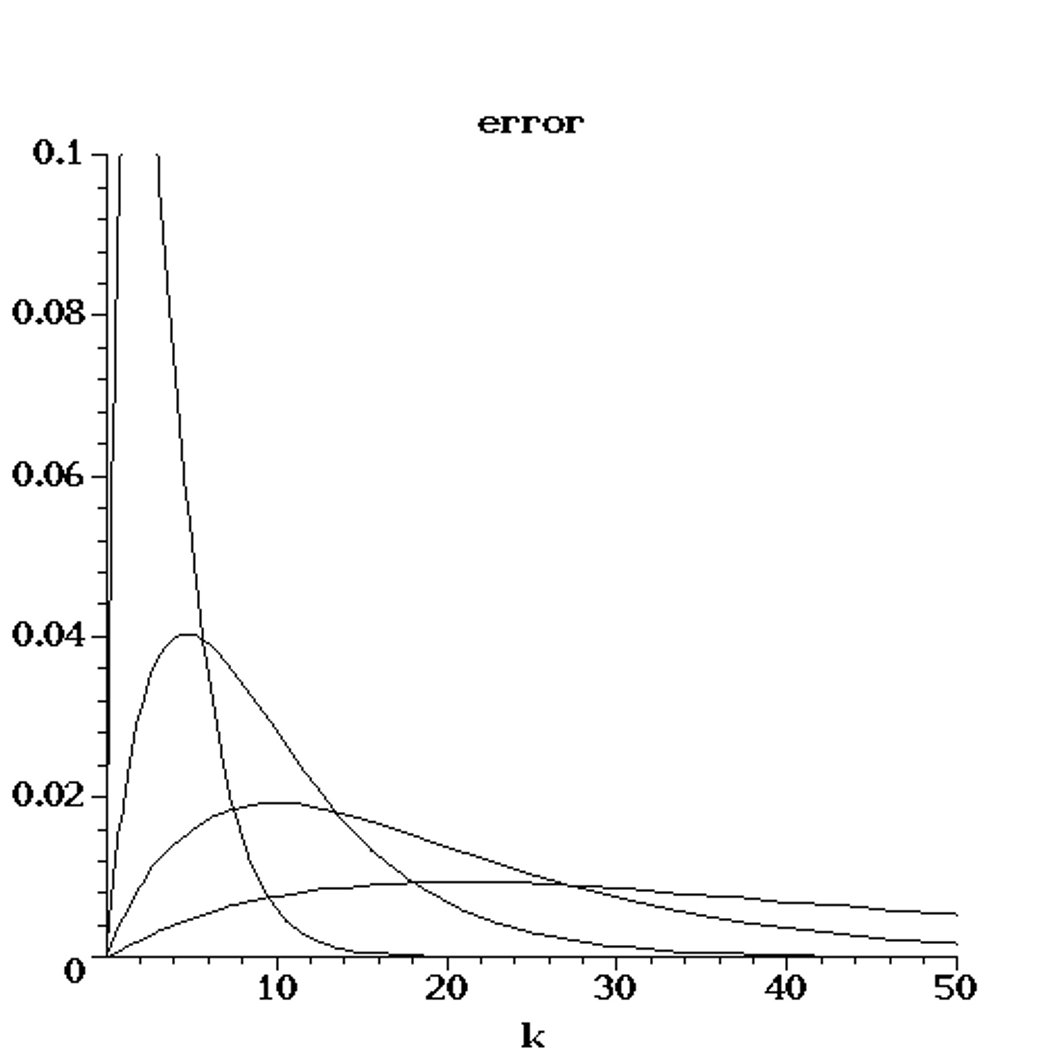
\includegraphics[width=0.25\textwidth]{Chapitres/PublicationsSample/Revue/fig1a.jpeg}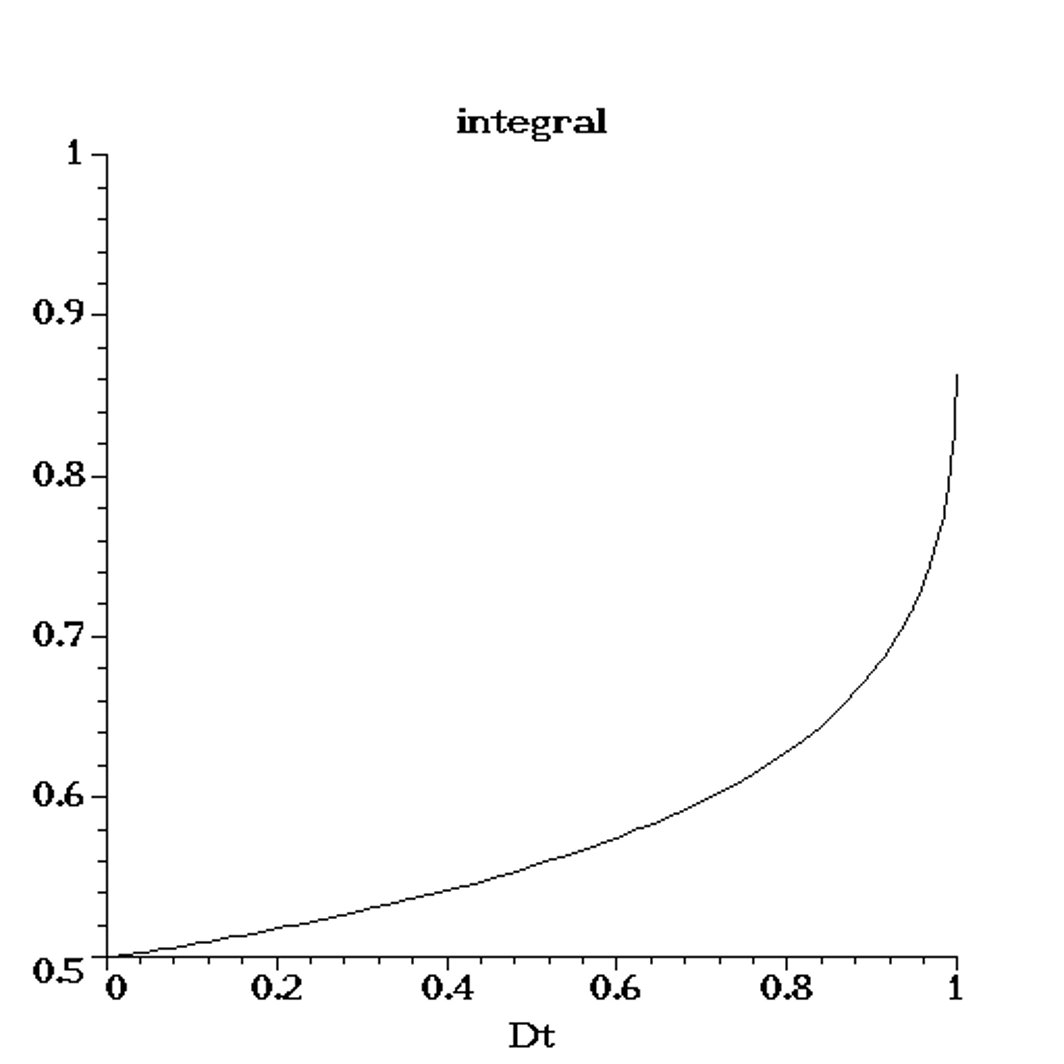
\includegraphics[width=0.25\textwidth]{Chapitres/PublicationsSample/Revue/fig1b.jpeg}\end{center}
\caption{{\em Left view}: The normalized bias temporal profile between the continuous scheme and its discrete approximation,
drawn here for $\Delta t / \tau_j = [0.05, 0.1, 0.2, 0.5]$ from the flattest to the sharpest curve respectively.
{\em Right view}: The integral of the bias along the trajectory as a function of $\Delta t / \tau_j$, making explicit that the cumulative bias is never negligible even for very small leak, while it diverges for large leak.
See text for details.}
\label{fig:euler-error} 
\end{figure} 
%%
In such a simple case,\footnote{In the scalar case, an explicit closed-form is automatically derived from a few lines of, e.g., {\tt maple} symbolic code:
\\{\tiny \tt \begin{tabular}{l}
eq := D(V)(t) = -W * V(t) + b: assume(0 < W, W < 1): \\
\# Continuous solution, assuming t0 = 0 \\
s\_c := dsolve({eq, V(0) = V0}, V(t)); \\
\# Euler approximate integration, assuming delta\_t = 1 \\
s\_e := rsolve({subs(eq, t = k, V(k + 1) = V(k) + Dt * D(V)(t)), V(0) = V0}, {V}); \\
\# Bias analysis \\
err\_k := simplify(factor((subs(s\_c, t = Dt * k, V(t)) \\
- subs(s\_e, V(k))) / (V0 - i / W)), {Dt * W = c}); \\
\end{tabular}}\\ while the result is straightforward to apply to the eigenvalue decomposition of the ${\bf W}$ matrix.
Furthermore, in the scalar case, 
if the Euler approximation is used with $Dt = (1 - exp(-W \, \Delta t)) / W = \Delta t - W/2 \Delta t^2 + O(\Delta t^2 )$ in numerical scheme,
the bias is canceled, which is not generalizable in the vectorial case since it depends on the leak value.
}
%%
both the continuous scheme and its discrete approximation starting from the same initial value converge towards the same fixed point (which can be found in all textbooks), but not though the same trajectory (which is surprisingly not studied in text books up to our best knowledge).  More precisely the bias in an eigendirection of the ${\bf W}$ matrix is proportional to $V_j(0) - I_j \, \tau_j$, where $1/\tau_j$ is the eigenvalue (i.e., the leak) in this direction, and follows a double exponential profile, only function of $\Delta t / \tau_j$, as illustrated in Fig.~\ref{fig:euler-error}. In words, the higher $\Delta t / \tau_j \in [0, 1[$ (this boundaries corresponding to the convergence interval), the higher the bias magnitude, but the quicker the bias between both methods vanishes.  The highest leak thus determines the maximal bias, the smallest leak the maximal duration of bias. \\

It is a counter-intuitive and very important result to notice that large leaks (i.e. small time-constants) indeed accelerate convergence, but with the drawback to generate large errors during the first iterations.  This means that the system dynamics may very easily switch from one attractor to another, at the beginning of the trajectory, even in such a very simple case.

\paragraph*{The general case: consequences}

In more general cases, there is no cute closed-form formula, as in the previous toy example, but it is obvious to infer to which extends the same kind of bias occurs.

In the non-constant case (i.e., leak, weights or currents vary with time), the previous results generalize considering bounds of the, now variable, leaks. 
In the non-linear case, the previous results generalize bounding the non-linear function $\sigma_j()$ by the corresponding maximal slope linear function.
See, e.g. \cite{Cessac:2007} for a review of such tools.
More precisely, if the system is hyperbolic, the same condition applies on the Jacobian of the system at any time and state value.

If the input variable $I_i(t)$ is not constant, we are thus in the situation where we track the true solution, and this is qualitatively equivalent to be reset at a new initial state at each step. As a consequence for small $\Delta t / \tau_j$ the system is expected to be always in a transient biased state with first iteration large errors, whereas for large  $\Delta t / \tau_j$ the system is always going to have a non-negligible lag with respect to the true solution. There is clearly a trade-off to find out, but always impaired by an incompressible bias.

As a consequence, we learn something from the present tiny analysis, even in more general cases: the method never converges at the trajectory level.
In any case, the cumulative bias is never negligible, with a lower bound for small leak, while diverging for large leaks.
This shows the very important difference between the fact that the discretization methods {\em converge at least} toward the expected fixed point 
and the fact that the simulation trajectory is unbiased. In the toy example, unbiasness never occurs, except in the singular case where $V_j(0) = I_j \, \tau_j$. Where stands the ``mistake'' ? At the implementation level, it stands on the simple fact that we are stick to synchronous computations.

\paragraph*{When asynchronism solves the situation}

At the implementation level, we obviously need several sampling times for a given simulation time in order to make the discrete approximation converge towards the continuous one,
which is often not taken into consideration. 

At the modeling level, the present mistake stands on the belief that a pertinent model of the reality has to be a ``continuous'' model, its discretization being a kind of second-class implementation detail. 
This is definitely wrong when modeling digital computational systems, but this is also questionable for microscopic neural models 
(see, e.g., \cite{Cessac:2008} for a discussion on biologically plausible generalized integrate and fire neuron models)
and mesoscopic neural map models (see, e.g. \cite{Rougier:2006} for a discussion at this modeling scale), 
the key question being ``what do we want to learn'' from the model or its simulation.

Now let us reconsider equation~(\ref{eq:DNF-discrete}) in the asynchronous computation paradigm. We have at time $t$, estimations of other units $\{\hat{V}_j(t)\}$, and estimations of the input $\hat{I}_i(t)$, and have missing values specified as a first approximation, as discussed in section~\ref{paradigm}. We thus can approximate:
%%
\begin{align}
\hat{J}_i(t) = \hat{I}_i(t) + \sum_{\substack{j \in M\\k \in \{k_{\min}, k_{\max}\}}} W_{ijk} \, \sigma_j\left(\hat{V}_j(t - k\, \Delta T)\right) \notag
\end{align}
%%
and are left with solving:
%%
\begin{align}
\frac{\Delta V_i(t) }{\Delta t}  = - L_i \, V_i(t)  + \hat{J}_i(t) \notag
\end{align}
%%
with the obvious closed form solution:
%%
\begin{align}
\label{eq:DNF-solution}
\hat{V}_i(t) = V_i(0) \, e^{-L_i t} + \int_0^t d\eta \, e^{-L_i (t - \eta)} \, \hat{J}_i(\eta)
\end{align}
%%
which is straightforward to iteratively approximate up to some adjustable time $t$, at any degree of precision, and easy to update as soon as better estimations of $\hat{J}_i(t)$ are available. Several further implementation choices are to be specified up to this point, but it is clear that all ingredients are there to design an asynchronous implementation of~(\ref{eq:DNF-discrete}).

\subsubsection{Value discretization issues}\label{dds}

A Discrete Dynamic System (DDS) is a finite set of elements, each taking a finite number of states evolving in a discrete time, by mutual interactions. In \cite {Robert:1994}, a book dedicated to the analysis of the temporal dynamics of such systems, Robert proposes a general framework, i.e., "a chaotic discrete iteration mode", to analyze such systems. The studied system is a cellular automaton with $N$ Boolean cells (a finite number of states), which may correspond, in a neural network, to an active neuron state (spiking) or a silent state. Each unit\footnote{More precisely, starting from an initial state at $t=0$, at each time step each unit updates its state function involving the states of the corresponding subset of elements, using any specific iteration mode (parallel, serial or chaotic).} is influenced by a subset of units that are involved in its update. 

Indeed, though a computer variable takes a finite number of values, the DDS results do not apply to floating-point number representations, because the order of magnitudes of the results are not usable in practice. Furthermore, DDS are not sufficient for modeling the targeted systems, i.e. DNF, that represent physical quantities, thus are best modeled by differential equations with continuous values. However, depending on the level of modeling, DDS could encounter for qualitative behaviors and we include them in the discussion in the sequel.


\subsection{Convergence and guaranty of computation}

Let us now report the proof of the convergence of asynchronous algorithms. We are in a {\em bounded asynchronous framework}, i.e. two main assumptions are required: \begin{itemize}
\item {\em bounded delays}. The delays should be bounded by a uniform finite constant $\Delta_{ij} \leq D < +\infty$. All sampling delays are thus finite.
\item {\em non starvation condition}. There is a maximal uniform bound $B$, between two updates for a given unit. Each unit should provide an update at least once during all interval of length $B$.
\end{itemize}
Different versions of these assumptions have been assumed in asynchronous computational algorithms like in \cite{Chazan:1969}. 
Therefore, with some additional conditions on the differential equations system (specially the leak function), uniform convergence at a geometric rate is proved. Let us precisely state the result.

Let us write ${\bf W}$ the weight matrix defined in~(\ref{eq:def-W}) in the case without transmission delay and when $\sigma_j(u) = u$. If transmission delays occur, ${\bf W}$ is now a tensorial quantity, and standard methods to rewrite the $n$th-order system as an augmented dimensional $1$st-order system are standard, ${\bf W}$ being a matrix in the augmented system. If the non-linearity $\sigma_j(u)$ is present, using differential inequalities, the non-linear system has to be bounded by a linear system of weight ${\bf W}'$. This is non trivial and beyond the scope of this short paper, and we refer to \cite{Mitra:1987} for a full development. Despite the technical difficulties, the underlying idea is quite simple: the weight has to be multiplied somehow by the highest slope of the non-linearity, i.e. $W'_{ijd} \simeq \sigma_j'(0) \, W_{ijd}$ for a sigmoid profile. Therefore, though not trivially, the following result holds in the most general case.

Based on this, if we refer to Mitra's work, our differential equation is a particular case of the proposed framework\footnote{It corresponds to equation (6.7i) of \cite{Mitra:1987}, with ${\bf D} = {\bf I}$ the (identity matrix) and ${\bf B} = {\bf W}$.}. Applying Proposition 2 of the paper, uniform convergence at a geometric rate in the asynchronous mode occurs when, in our case, ${\bf I} - |{\bf W}|$ is an M-matrix (i.e. a matrix whose off-diagonal entries are less than or equal to zero, with eigenvalues whose real parts are positive).
Since ${\bf W}$ is a symmetric positive matrix, thus diagonalizable, with positive eigen-values, ${\bf I} - |{\bf W}|$ is a M-matrix a soon as these eigen-values are smaller than one.
As a consequence, we can conclude that asynchronous computation convergence in such a neural network is guaranteed and that the long-term average rate geometric convergence (per update) is not less than:
%%
\begin{align}
\label{eq:convergence}
\frac{1}{\tau_{\min}} \leq \frac{1}{D + B}
\end{align}
%%
where $1/\tau_{\min}$ is the spectral radius of ${\bf W}$, i.e., the largest (here positive) eigen-value corresponding to the smallest combined leak of the system. This is a very precise and effective result, {\em with a usable number}.

The main problem, even if the system is finite and time is discrete, is not only to ensure the convergence to a stable state (this obtained here, if the system is contracting), but to guaranty the computation is going to converge to the right result. Here is the power of the Mitra result. In the non-linear case, Mitra has thus to assume that the non-linear functions are continuous (but not necessarily smooth) and bounded by a linear contracting function, to obtain the same result. In our case, this means that the non-linear, so-called sigmoid function $\sigma()$ can not be a step function, but any usual continuous profile is convenient.

\subsubsection*{Convergence when values are discretized}

A step further, let us discuss what can be stated, when values are also discretized.
In the numerical analysis community, the  reference book in both continuous and discrete context is Bertsekas and Tsitsiklis book, 
chapters 6 and 7 \cite{Bertsekas:1997}, released in 1989. It presents some algorithms and gives sufficient conditions for convergence for general nonlinear problems and necessary conditions for linear problems. 
In the special case of discrete dynamic systems without transmission delays, the main result presented in \cite{Robert:1994,Bahi:2002}, is that if a system is pseudo-periodic, it converges at most after $N$ pseudo-periods. A pseudo-period corresponds to a sequence of events in which each unit is updated at least once. So with only $N$ synchronization points the system convergence is guaranteed. 
But when we introduce transmission delays and continuous variables, such an assumption is no more valid, thus does not ensure the convergence. 

\subsubsection*{An illustrative example}

Let us consider for example a two-layer network, each layer being of size $N \times N$ units. 
An input layer corresponding to the constant current entry is feeding an output layer. 
Each unit of index $i$ of the output layer receives its input $I_{i}$ from the input layer with respect to a receptive field (a Gaussian connection). 
We suppose that there is neither lateral connection nor feedback in the input map. Lateral connections in the output map are excitatory, decreasing with distance and the input is inhibitory (the reverse connectivity scheme is also suitable). It means that each neuron in the output layer is excited by its neighbors and inhibited by the neurons in its receptive field. The resultant activity in the output map is a difference of Gaussian which is a computation scheme very used in dynamic neural networks.


So, in this case, for each unit of the $M = N \times N$ units, equation~(\ref{eq:DNF-discrete}) writes with weights $W_{i=(u,v)\,j=(u',v')\,d}$ indexed in function of the 2D geometry of the network and $V_{i}$ stands for the membrane potential, $W_{ijd}$ is a positive symmetric tensor in this case, and $I_{i}$ is the constant current input, projection from the input layer. One instantiation, without delayed weight, would be to choose:
%%
\begin{align}
W_{ij0} = a_+ \, e^{-\frac{|i - j|^2}{v_+^2}} -  a_- \, e^{-\frac{|i - j|^2}{v_-^2}} \notag
\end{align}
%%
then as a side result of the work reported in \cite{Alexandre:2009}, we can state:
%%
\begin{align}
\frac{1}{\tau_{\min}} \simeq \sqrt{\pi} \, (a_+ \, v_+ - a_- \, v_-) \notag
\end{align}
%%
the approximation being to neglect the finite side effect of the corresponding 2D map. 
Then, combined with~(\ref{eq:convergence}), we have a concrete bound on asynchronous convergence.\\

As soon as the {\em sampling} and {\em simulation} times are not mixed, and the dynamic neural field dynamics attractor is a fixed point, attained with or without damped oscillations, any general asynchronous relaxations schemes with neither unbounded transmission delays, nor starvation, uniformly converge at a geometric rate. This result has obviously no reason to hold for more complex dynamics, especially in chaotic cases, since even a negligible error is going to make the discrete approximation diverge exponentially fast, without any chance to redress the error by a bounded number of asynchronous relaxations.  In the case of a periodic stable attractor, though the previous formalism can not be applied as it is, it seems reasonable to assume that the asynchronous relaxations would be able to maintain the discrete approximation scheme at a bounded error of the continuous exact solution. Thanks to this fundamental result, we can consider the synchronous/asynchronous dynamical neural fields simulation dilemma, (i.e., the fact that authors often wonder whether they can efficiently simulate such a dynamical system using an asynchronous scheme) as solved in such a context.

\subsection{A generic asynchronous implementation}

Let us finally consider a last aspect of asynchronous computation, i.e. not the fact that we want to simulate a continuous system in an asynchronous way, but the fact that we want to simulate a system {\em intrinsically asynchronous} in a sequential or distributed computational device.  This covers two fundamental aspects.  On one hand, each unit has a local clock, so the state evolution depends entirely on the occurrence of asynchronous mechanisms over time.  This means there are delays between units, with unpredictable exact values.  On the other hand, there is another semantics related to anachronism, i.e. the fact that information associated to input and output is defined by both a value and the time at which the value is issued.  In other words, the information is defined through temporal events.

Concerning biologically plausible models, the event-driven computation scheme has been mainly developed for spiking neuron models.  Such models are not addressed here \footnote{see \cite{Gerstner:2002} for an introduction and \cite{Cessac:2008,Cessac:2010} for a recent theoretical analysis and general discussion in link with these aspects}. Nevertheless, this scheme could be certainly extended at a more mesoscopic level, as that of cortical columns, modeled by dynamical neural fields, as developed here. The dedicated simulation tool is an event-based neuron simulation kernel as proposed by, e.g., \cite{Rochel:2003} based on the well-known Discrete Event System Specification (DEVS) framework (for a comparative review see \cite{Brette:2007}), very easy to simulate on a single processor.\\

Very concretely, each unit is defined by three functions: (i) The next event function provides an estimation of a lower-bound of the future time, where the next event time is going to be fired. (ii) Two update functions define how the unit update its state when either its own internal event, or another incoming external event is issued. The DEVS allows to show that given this specification, a complete asynchronous system can be simulated, using a simple calendar queue of events, on any device (see, e.g., \cite{Cessac:2009} for details). This allows not only to simulate asynchronous calculations on a centralized system, but also to {\em mix} both kinds of implementation. 

In brief, we propose to not only use event-based unit simulation at the microscopic level, targeting spiking-neurons, but also at the mesoscopic level, modeling the emergence of temporal events (synchronization or more complex mesoscopic spiking patterns, dynamic change triggering, etc..).

\subsubsection*{An illustrative example}

Let us instantiate this general discussion, through an illustrative example. In a recent work \cite{Rougier:2006} a model has been designed that performs global competition, only using local connections, with diffusion of the inhibition throughout the network. This is far quicker to have a few local interactions when computing activity within the network and this makes the model a real candidate for distributed computations.
We have re-implemented this mechanism considering asynchronous sampling via a minimal event-based simulation 
kernel\footnote{Code available at {\tt http://enas.gforge.inria.fr},
while {\tt EnaS} is the general purpose large-scale event-based multi-scale simulator at the edge of the state of the art.},
which obviously works since the system is still contracting when using asynchronous sampling, as discussed previously. 
This has been numerically experimented, as shown in Fig.~\ref{fig:bump}, 
with the obvious heuristic to have the local sampling period roughly proportional to the state value variation (parsimonious principle),
with a strong robustness with respect to the related parameters (modifying the asynchronous paradigms changes the transitional values, slightly influences  the convergence speed, but does not modify the final result).

This numerical result corresponds to trivial implementation of~(\ref{eq:DNF-solution}), so that the convergence is really obtained thanks to asynchronous paradigm. We have numerically verified on this simulated example that we could approximate the true solution at any precision (which was obviously expected anyway). Though this is not informative to report in details, we have been able to reproduce all qualitative DNF input/output functions ({\em filtering} of the output bump shape, {\em selection} of the output bump among several input bumps, {\em tracking} of a moving input bump at the output level, {\em remanence} of the output bump after the partial or total suppression of the input bump, see \cite{Alexandre:2009} for details). We have been able to verify that providing that~(\ref{eq:convergence}) is verified, the computation was guaranteed in all observed cases while if far away from this bound, it is expected to fail. It is however still an open point to verify whether this bound is numerically a thick one, in all interesting case.
%%
\begin{figure}[ht]
\centerline{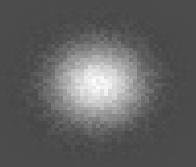
\includegraphics[width=0.25\textwidth,height=0.25\textwidth]{Chapitres/PublicationsSample/Revue/fig2a.jpeg}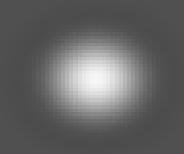
\includegraphics[width=0.25\textwidth,height=0.25\textwidth]{Chapitres/PublicationsSample/Revue/fig2b.jpeg}}
 \caption{An example of asynchronous sampling of such maps (event-based implementation), applying convergence criteria derived here.  We have numerically verified the conjecture that the present results apply when using asynchronous sampling.  {\em Left view}: intermediate result, the fact asynchronous sampling yields randomization is visible.  {\em Right view}: final result, after convergence.}
\label{fig:bump} 
\end{figure}
%%
Though this is only a preliminary result that opens large perspectives on new asynchronous paradigms for discrete neural field implementations.

\subsection{Discussion and conclusion}

This work aimed at addressing the following key-points: 
%%
\begin{itemize}
%%
\item Making the difference between the discretized model {\em sampling} time and the implementation {\em simulation} time (several implementation steps may be use to iteratively estimate one sample of time, whereas a closed-form expression may provide the result after several sampling times in one simulation time).
%%
\item Calculating the bias between a continuous stable trajectory and its discretized approximation, all along the trajectory and given a sampling time (not only be sure that either the asymptotic targets are the same or that everything is perfect if the sampling is infinitesimally small).
%%
\item Making explicit the goals of using synchronous/asynchronous mechanisms at both the modeling level (asynchronous evaluation mechanisms avoid generating spurious synchronizations not present at the modeling level) and the implementation level (simulation on coarse or fine grain parallel processing clusters to multiply the calculation capability). 
%%
\item Specifying whether not only the calculation but also the time is distributed (global time versus local time), i.e. whether a discrete clock dynamic system versus a discrete event dynamic system is considered.
%%
\item Deriving, in the case of the general family of dynamic neural field distributed and interconnected units, quantitative bounds that guaranty the convergence of the implementation calculations towards the modeling expected solution.
%%
\end{itemize}
%%
Addressing all these issues in such a short review would have been unrealistic, whereas a major but rather unnoticed work \cite{Mitra:1987} on asynchronous computing, addresses these issues at a very general and deep level. The goal of this paper was thus to apply these results to the case of DNF computations and provide the complements in order to make these results directly usable.\\

Making the explicit distinction between sampling times and simulation times allowed us to review how well-established asynchronous evaluation methods can be efficiently used for dynamic neural fields simulation; as soon as reasonable assumptions are verified, fast convergence and unbiasedness are guaranteed. In return, as we explained in the previous section, dynamic neural field theory provides a fruitful playground for the study of asynchronous evaluation schemes. For example, in \cite{Rougier:2006}, it has been shown (numerically) that such an asynchronous evaluation method leads to new stable solutions that are functionally different from the continuous case. When presented with two identical stimuli at different locations, the field is able to stabilize itself on either one of the two stimuli because of the perturbation that lead the system away from a very unstable equilibrium state (like would also do any kind of noise). However, this new state, that has been shown to be very stable, can be also easily proved not to be a solution of the continuous equation of the field. What is thus the relevancy of such a continuous description if we are to evaluate it using numerical asynchronous equations ? Ideally, we wish we could have an equivalent continuous asynchronous description but unfortunately, this is not yet the case in the field of mathematics. We should then take extra precaution when describing a system using continuous equations and wonder if we are really simulating what we advertised in the definition of the system. Particularly, at the mesoscopic modeling level, it may be worthwhile to use an event-based paradigm instead of a clock-based one, as it is a well-defined paradigm which takes into consideration that not only the processing but also the timing are fully distributed.\\

From a more cognitive point of view, this study reveals the implicit presence of a central clock in a number of models and thus the implicit presence of a grand supervisor (a.k.a. central executive, homunculus, etc.) orchestrating the overall activity of the model. While this may be acceptable in most models that do not care about this parasitic presence, it is hardly acceptable if a model pretends to vanquish the curse of the homunculus.




%\section*{}
\paragraph{Acknowledgment.} Partially supported by the ANR MAPS \& the ANR KEOpS projects.

%\bibliographystyle{elsarticle-harv} {\scriptsize \bibliography{biblio.bib}}

\section{Visual Target Selection Emerges from a Bio-inspired Network Topology}
\begin{center}
Wahiba Taouali, Nicolas Rougier et Fr\'ed\'eric Alexandre\\
Studies in Computational Intelligence, pages 317--330.\\
\end{center}


\paragraph{Abstract}
%The abstract should summarize the contents of the paper and should
%contain at least 70 and at most 150 words. It should be written using the
%\emph{abstract} environment.

 \textit{The orientation of sensors toward regions of interest of the
  environment is an important motor activity, monitored by ancient
  structures of the brainstem. Particularly, the superior colliculus
  is known to be deeply involved in visual saccadic behavior. Target
  selection relies on various hints including exogenous information
  about the nature and the position of candidate targets and
  endogenous information about current motivations. We present a model
  of the collicular structure based on biological data, the
  specificity of which is related to the homogeneity of the underlying
  substratum of computation. This makes it more suitable to process
  massive visual flows on a distributed architecture, as it could be
  requested in a realistic task in autonomous robotics. The present
  model is restricted to the exogenous part of the visual pathway,
  from the retina to the superior colliculus. A realistic behavior for
  the selection of exogenous targets is reported here.}

%---------------------------------------------------------------------------

\subsection{Introduction}

Displaying an intelligent behavior is often synonymous of
intelligently exploiting the surrounding environment. In many animals,
this is massively performed through the analysis of information by the
visual channel, to orient subsequent behavior (perceptual decision and
action). Much research in computational intelligence aims at endowing
animats with such powerful skills, drawing inspiration from the living
science, at several levels of description. At the functional level, it
is important to know which information animals extract from the visual
input, possibly in parallel communicating processing flows and,
accordingly, which representations are built and exploited in memory
systems. At the physiological level, if one wishes a deep anchoring in
biological inspiration, the functional behavioral analysis has to be
mapped onto the neural substratum and its known anatomy and
physiology, which can also give indications about the way behavioral
properties can emerge from fine grained neural computations. At the
operational level, a formalism of computation has to be defined to
implement the corresponding models, as a compromise between accuracy
to biological inspiration and efficiency of computation for animats
plunged in the real world.

\subsubsection{At the functional level}

It has been proposed for a long time \cite{Ungerleider:1982} that two
separate visual systems can be described in the ventral (temporal) and
dorsal (parietal) visual cortex. These associative cortical areas
were first respectively presented as dedicated to identification and
location of objects. Later \cite{Milner:1995}, it was more precisely
explicited that the ventral cortex elaborates the construction of the
perceptive representation of objects in the world, thanks to its
privileged relationships with the limbic system, center of the
declarative memory, whereas the dorsal cortex, linking the primary
visual cortex and the motor cortex, allows for the visual control of
actions towards that objects, by extracting, in the visual flow,
information useful for the preparation of actions (eg. size of an
object for anticipating the size of the grip in a grasping movement). 

In \cite{Goodale:1998}, the authors explain that both cortical axes
are separate but deeply interacting in primates and conclude that this
dual view reconciliates the reconstructionist approach by D. Marr, very
much influential in the domain of computer vision, and the
purposive-animate-behaviorist approach by J. Gibson, very popular in
reactive robotics.  Particularly, the interplay between both
functional analysis is well illustrated by two adaptive behaviors that
allow to decrease the huge amount of information brought by the visual
channel: visual attention proposes a sequential processing of possible
targets; saccadic movements orient the body and particularly the fovea
on regions of interest in the visual scene. In both cases, the visual
control of action is dedicated to elaboration of a flexible and
powerful representation of the visual information. According to
\cite{Ballard:1997}, fixation and attention can be considered as
mechanical and neural deictic devices and the authors explain the
computational power of such a technique for variable binding and other
strategies of embodied representation. At the cerebral level, the
premotor theory of attention \cite{Rizzolatti:1987} stipulates that
there are common processes between these key behaviors and, more
precisely, that they share common neuronal circuits: Attention would
be pre-programming of a saccade.

\subsubsection{At the physiological level}

In the above mentioned paper \cite{Goodale:1998}, the authors also
make a very precious reference to phylogenesis and indicate that, in
more primitive animals, the goal of vision is not to see but to guide
their movements. The visual control of actions corresponds to a direct
instantaneous perception system, whereas the identification of objects
can be seen as a relation from the present visual input to a past
information stored in declarative memory, not present in ancient
species (eg. reptilians, amphibians). Consequently, the general
purpose network that we observe in the brain of primates, where the
cortex plays a major role, must be also related to the basic visual
system of a frog \cite{Lettvin:1968}, where only several input/output
sensorimotor lines (predator avoidance, prey catching, locomotion
guiding) define a kind of purposive vision. The very nature of the
evolution of the brain makes that these ancient visuomotor structures
are still present, though modulated of course by advanced control
systems and coordinated by more recent memory systems.

Particularly, these circuits converge, in the frog, in a neural
structure called the tectum, directly linking retinal inputs to motor
actions. In mammals, the similar structure is called the superior
colliculus (SC).  Indeed, this small structure in the midbrain of
mammals is known to be implicated in these sensorimotor
behaviors. From an hodological viewpoint, it integrates visual
information from many sources (cortical or not) in the brain and sends
projections toward the brainstem premotor circuits that trigger
saccades \cite{Isa:2002}. From an anatomical viewpoint, it consists of
a set of topological maps, mapping the surrounding space, from visual
to motor reference frames \cite{Girard:2005}. And from a physiological
viewpoint, its inactivation or electrical stimulation confirms its
role in visual attention and saccades \cite{Muller:2005}.

Many models have studied the SC and associated properties
(cf. \cite{Girard:2005} for a review). We just mention here some models
underlying the link to information flows and underlying behavior. The structure
of the model described in \cite{Findlay:1999} underlines that the main task is
to decide when and where the saccade must be performed. As a consequence, two
hierarchical axes are defined. The When axis (corresponding to the FEF (Frontal
Eye Field) area in the prefrontal cortex) decides when to leave the current
fixation point, whereas the Where axis corresponds to the SC and implements a
spatial competition between candidate targets. A double-axis model combining
FEF and the SC is also proposed in \cite{Kramer:1999}, to explain the
integration of exogenous elements (external stimuli coming from the retina to
the SC) and endogenous elements (internal expectancies or instructions
elaborated in the prefrontal cortex). Later on, \cite{Godijn:2002} proposed a
competitive integration model based on strong experimental evidences at the
behavioral level, indicating that all these elements (spatial vs temporal
processing and integration of exogenous vs endogenous stimuli) can be
integrated in a unique map, seen as a model of the SC. This common saccade map
also includes features generally reported as physiologically plausible in the
SC: a local excitation in the map allowing to combine close stimuli and a wider inhibition mechanism to trigger a competition between far stimuli. This
interaction scheme explains why it was possible to use such a formalism as
Dynamic Neural Field (DNF) \cite{Amari:1977} to implement this kind of model, as it is also the case in \cite{Trappenberg:2001,Schneider:2002}.

\subsubsection{At the operational level}

Many recent models of the SC explain a wider range of visuomotor and more
generally cognitive functions at the price of a more complex internal circuitry
describing the SC. Indeed, those models define several kinds of units,
depending on their location on the map, which is not very consistent with the
principle of homogeneity in DNF. More precisely, in \cite{Trappenberg:2001},
the reported behavior is obtained with some units standing for the currently
fixated stimulus (consequently in the fovea), other units representing
potentially fixated stimuli in the periphery, both kinds sending inhibition to
other units triggering saccades toward a target. These kinds of units, also
exploited in the model by \cite{Schneider:2002}, are presented as representing
respectively so-called fixation, build-up and burst neurons, which are
sometimes reported as parts of the intermediate layer of the SC
\cite{Wurtz:1994}, though this is still to be clearly established. In
\cite{Godijn:2002} also, the substratum of computation is not homogeneous,
since the sensitivity of units decreases with their eccentricity onto the
map. This trick is used to reproduce the observation that the latency of a
saccade toward a target, presented together with a distractor, is longer when
the distractor is closer from the rostral zone of the SC (corresponding to the
fovea).

Consequently, these complex models often rely on physiological considerations
that are controversial and their inner mechanisms can often be described as ad
hoc, designed to stick to experimental observations. Moreover, this additional
complexity is often obtained by introducing numerous parameters, which affects negatively the
robustness of these models. Also, it becomes difficult to simulate
on-line the analysis of a visual flow, due to the amount of generated
computations. Such an assessment is contradictory to the ordinary view that
neuronal structures are often homogeneous, due to the repetitive tiling of
elementary circuits of neurons. It is also contradictory to the spirit of DNF
that have been designed as a generic homogeneous model for such populations of
neurons.  For that reasons, in this paper, we present a model of the SC, based
on DNF formalism, with an identical functioning rule for all the units in the
map. Moreover, obtaining such an homogeneous substratum can yield fully
distributed computation, which is important to design models that can be used
online in robotic visuomotor tasks. Also, this approach has a common ground
with the reactive and enactive frameworks mentioned above, which state that
fundamental properties can emerge from low-level, basic computations and not
from a high-level structured module. Correspondingly, one of our questions here
is to observe which of the known properties of the SC we can obtain with such
an homogeneous and simple brick of computation.

Finally, the proposed model is not an isolated structure but is a function of
exogenous information flows and associated geometrical properties.  We have
explained that the SC is undoubtedly an important integrative structure, to be
included in a cognitive neuroscience modeling approach of visuospatial
behaviors and we will illustrate accordingly how this model could be exploited
in more high level tasks.



%---------------------------------------------------------------------------
\subsection{Model}
The computational paradigm supporting the model is grounded on the
notion of a unit that is essentially a set of time dependent values
varying under the influence of other units via learnable weighted
links (fig. \ref{fig:group}).  The evolution of units' value is
defined by a set of differential equations expressed in standard
mathematical notations. The units are organized into groups that form
a network and each unit can be linked to any other unit (including
itself) using a weighted link. The modeling framework\footnote{See
  \url{http://dana.loria.fr}} offers a set of core objects needed to
design and run such networks. However, in this framework, what is
actually computed by a unit and what is learnt are the responsibility
of the modeler who is in charge of providing the equations governing
the unit's behavior and the plasticity of its links.
%%
\begin{figure} %[htbp]
  \begin{center}
    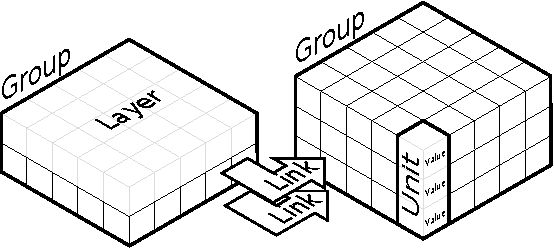
\includegraphics[width=\textwidth]{Chapitres/PublicationsSample/Chapitre/figures/group}
  \end{center}
  \caption {A unit is a set of one to several values ($V_i$). A group is a
    structured set of one to several homogeneous units. A layer is a subset of
    a group restricted to a unique value $V_i$. A layer is a group. A link is a
    weighted connection between a source group to a target group. A group can
    be linked to any other group including itself.}
  \label{fig:group}
\end{figure}
Such a modeling framework is actually strongly constrained and cannot cope for
example with standard artificial neural networks. It is indeed centered around a
set of four principles (distributed, asynchronous, numerical and adaptive) that
we think may help to bring insights on our understanding of computational
intelligence. While many computational models involve explicit symbols and/or
a central supervisor, this framework is able to guarantee to a certain extent
the absence of such artifacts. In the end, what is achieved by such a model is
the sole result of the interaction of many units working together.


\subsubsection{Model architecture}
In short, we consider here projections to the SC coming from the
retina and the primary visual cortex, carrying exogenous information,
and not those coming from the frontal cortex, carrying endogenous
information.  Under that restriction, we want to check to what extent
the model exhibits some of the well known properties of saccadic
behavior associated to the SC. More specifically, our goals are to
analyze the topology of the visual information that we obtain after
applying this very simple transformation, together with the associated
behavioral properties. 

Consequently, the model is made of three distinct groups (see
fig. \ref{fig:model}) modeling the visual pathway from the retina (R)
to the superior colliculus (SC) through the primary visual cortex
(V1):
%%
\begin{itemize}
  \item retina (R, $256\times 512$ units) receives visual input from a CCD
    camera.
  \item visual cortex (V1, $256\times 256$ units) implements the actual
    cortical magnification.
  \item superior colliculus (SC, $63\times 63$ units) is the place where
    salient locations enters competition.
\end{itemize}
The retina model is restricted to the right visual field as it is known to be
the case in mammals visual pathway (left visual field projects to right
colliculus and right visual field projects to left colliculus). We used an
image size of $512 \times 512$ pixels and fed the retina with a normalized
gray-level image of size $512 \times 256$ pixels.
%%
\begin{figure} %[htbp]
  \begin{center}
    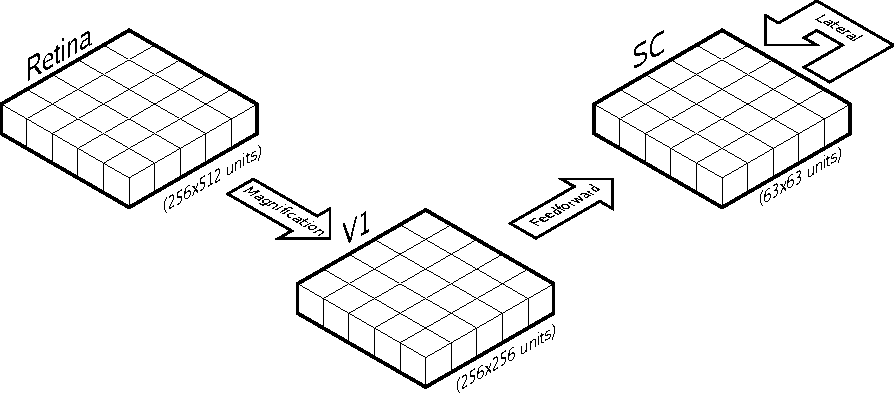
\includegraphics[width=\textwidth]{Chapitres/PublicationsSample/Chapitre/figures/model}
  \end{center}
  \caption {The model is made of three distinct groups. The retina receives
    input from a CCD camera and transmit information to the primary visual
    cortex where the actual magnification occurs. This result is then feed to
    the superior colliculus where salient locations enter competition.}
  \label{fig:model}
\end{figure}
%%
We will now detail the cortical magnification occurring between the retina and the
primary visual area V1 as well as the competition occurring within the superior
colliculus resulting in a unique localized packet of excitation designing the
selected target.

%---------------------------------------------------------------------------
\subsubsection{Cortical Magnification}
The retina represents the sensory input space and possesses a complex structure
composed of several layers of neurons. Vision actually starts early in the
layer of photo-receptors from where the flow of information is processed via
the ganglion cells which are large nerve cells whose cylindraxes form the optic
nerve. Due to the non-homogeneous repartition of photo-receptors on the (human)
retina surface, visual acuity decreases from the center of the retina (fovea)
to its periphery. This property is attributed to a variation in the density of
photo-receptors that decreases from the center to the periphery
\cite{Marilly:1999}. Consequently, the foveal region benefits from a much
higher resolution than peripheral regions and this property is preserved along
the visual pathway up to early visual areas \cite{Purves:2004}. This is
referred to as {\em cortical magnification}. To analyze this magnification in a
quantitative way, a coordinate system is often defined in the visual field. The
coordinate system that is best suited to the visual system is the polar
coordinates $(\rho,\phi)$. It characterizes a position in the visual field by
its eccentricity $\rho$ from the center of gaze and its polar angle $\phi$ is
measured, for example, in relation to the lower vertical meridian. We can
therefore define a retinotopic map which corresponds to the spatial
transformation of the image by the spatial arrangement of the grid of
neurons. It is often approximated by a log-polar transformation of the
spherical image centered on the eye \cite{Robinson:1972}. We used a simplified
model of the retina considering only the photo-receptors layer. And for
computational reasons (speed), we did not enforce the non-uniform repartition
of photo-receptors on the retina surface. Instead, we modeled a uniform
distribution of neurons onto the retina associated with a deformed polar
coordinate system as proposed by \cite{Ottes:1986}. Each cortical visual cell
is supposed to be connected to a single or several photo-receptor cells, with
respect to a logpolar deformation, that form its receptive field. So the non
uniformity is caused by the changing size of the receptive fields. We used
equations mapping retinotopic polar coordinates $(\rho,\phi)$ onto V1 Cartesian
coordinates $(\mathbf{x},\mathbf{y})$. These equations were first introduced by
\cite{Ottes:1986}:
\begin{eqnarray}
  \mathbf{x} &=& B_x \ln{(\frac{\sqrt{\rho^{2}+2A\rho|\cos{(\phi)}|+A^{2}}}{A})}\\
  \mathbf{y} &=& B_y \arctan{(\frac{\rho \sin{(\phi)}}{\rho|\cos{(\phi)}|+A})}
  \label{eq:magnification}
\end{eqnarray}
with $A=3^\circ$, $B_x=1.4mm$, $B_y=1.8mm$. These parameters have been chosen
to fit the stimulation map of the SC given by \cite{Robinson:1972}.  A neuron
in the visual cortex fires an action potential when a visual stimulus appears
within its receptive field. But for any given neuron, it may respond best to a
subset of stimuli within its receptive field corresponding to its preferred
direction. Neurons with similar tuning properties (what the neurons respond to)
tend to cluster together but the exact structure is still unclear. Then, it is
acceptable to assume that V1 has a retinotopic map similar to the collicular
motor map in \cite{Bear:1996}. It means that a cell at a given position
$(\mathbf{x},\mathbf{y})$ in the V1 map is activated by retinal cells in
positions ($\rho$, $\phi$) according to given equations. One result of this
deformation is that the same stimulus causes a large activation in the V1 map
if it is located near the fovea and smaller activation in peripheral positions
(cf. figure \ref{fig:magnification}).
\begin{figure}[htbp!]
  \centering
    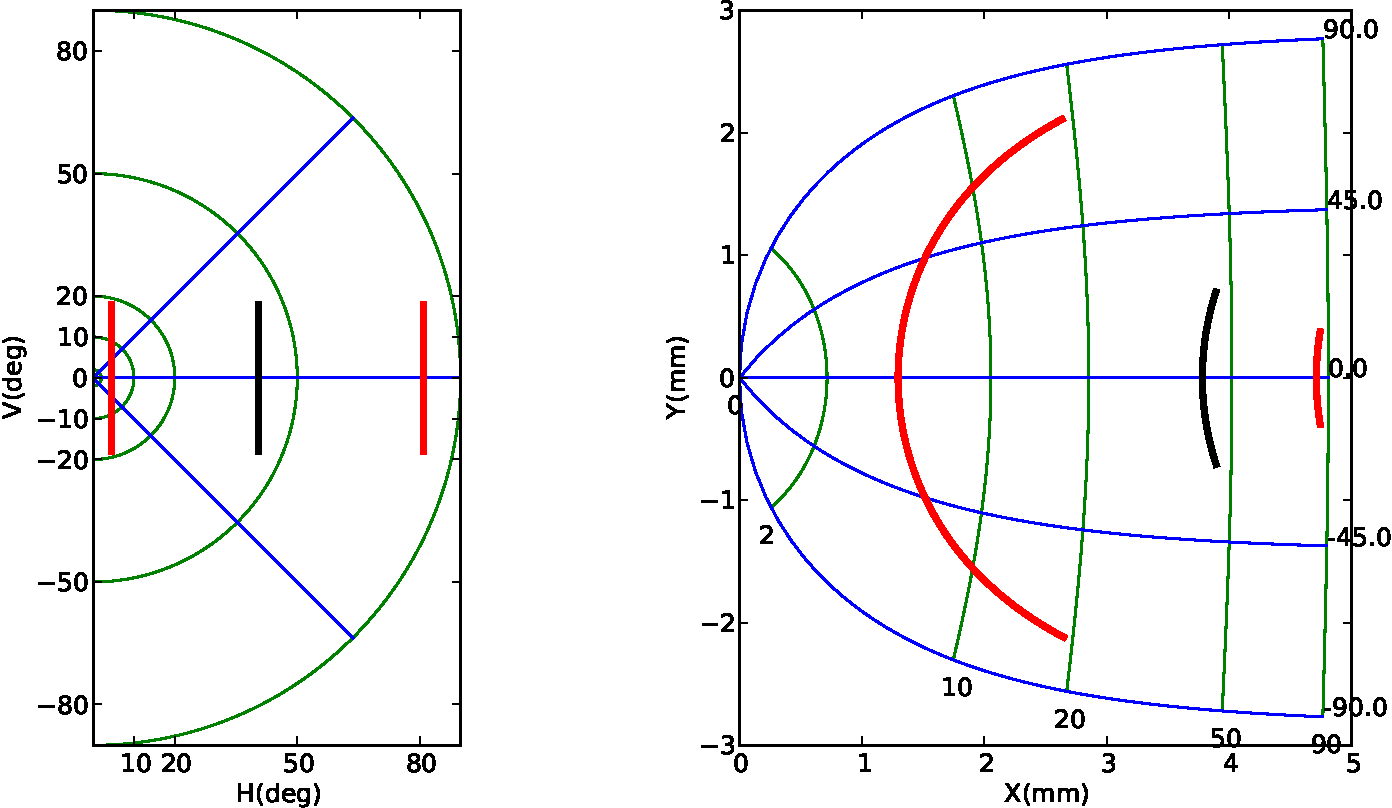
\includegraphics[width=\textwidth]{Chapitres/PublicationsSample/Chapitre/figures/mapping}
  \caption{Cortical magnification from the retina to the visual cortex distorts
    geometrical properties of the image while keeping neighborhood
    relationship.}
  \label{fig:magnification}
\end{figure}
Visual receptors of V1 have been modeled in two dimensions corresponding to an
eye visual hemifield with no connection between the different receptors.

%---------------------------------------------------------------------------
\subsubsection{Dynamic Neural Field Theory}
Collicular population (the motor layer of one superior colliculus) has been
modeled with respect to the dynamical neural field theory
\cite{Wilson:1973,Amari:1977,Taylor:1999} that describes the evolution of a
neural population using equation (see \cite{Rougier:2006} for details):
\begin{equation}
   \tau \frac{\partial u(\mathbf{x},t)}{\partial t} = -u(\mathbf{x},t) +
  \int w(\mathbf{x} - \mathbf{y}) f(u(\mathbf{y})) d\mathbf{y}\\
 + h + I(\mathbf{x}, t)
    \label{eq:dnf}
\end{equation}
where $\mathbf{x}$ denotes a location onto the SC; $t$ is time; $u(\mathbf{x},
t)$ denotes the membrane potential of a neural population at point $\mathbf{x}$
and time $t$; ${\tau}$ is the temporal decay of synapses, $f$ is a sigmoid
function computing the mean firing rate, $w$ is a neighborhood function,
$s(\mathbf{x})$ is the input received at position $\mathbf{x}$ and $h$ is the
mean neuron threshold. $w$ has been set as a difference of Gaussian ($DoG$) with
short-range excitations and long range inhibitions following anatomical and
physiological data as reported in~\cite{Munoz:1998}:
\begin{equation}
  \label{eq:DoG}
  w ({\bf x}-{\bf y}) = 
    A e^-{\frac{\vert {\bf x} - {\bf y} \vert^2}{a^2}} -
    B e^-{\frac{\vert {\bf x} - {\bf y} \vert^2}{b^2}}
\end{equation}
and $f$ has been set as a simple rectification of ${\bf x}$. The input
$I(\mathbf{x},t)$ is a direct one-to-one relationship according to V1 and SC
respective sizes.





%---------------------------------------------------------------------------
\subsection{Results}
The reported experimental results are of three kinds. Firstly, we
check that basic properties of information encoding are ensured
(topology, accuracy). Secondly, we examine the resulting saccadic
behavior for target selection from exogenous information, particularly
depending on the position of candidate targets with regard to the
fovea. Thirdly, we address more difficult cases, particularly
considering natural images and introducing the need for endogenous
information.

%---------------------------------------------------------------------------
\subsubsection{Output Decoding}
One of the questions related to the superior colliculus concerns the proper way
to decode the output. Since the amplitude and direction of a saccade depend on
the activity of the neural population in the deep SC \cite {Sparks:1990},
different ways of SC output evaluation have been proposed in the past:
\begin{itemize}
\item winner-take-all where the most active site indicates the direction
\item summation\cite{McIlwain:1976,Sparks:1976} where all activities of active
  neurons are summed with weights determined by their individual labels
\item weighted average \cite{Lee:1988} using a normalization
  according to the number of active neurons
\end{itemize}
These three evaluation schemes are equivalent in the case of a
normally activated population but differ when there is a deactivation
or an over-activation of a part of the population. We have retained
the last decoding scheme because the superior colliculus was modeled
using a dynamic neural field and it is thus ensured that a stereotyped
activity profile emerges anytime corresponding to the most salient
location of the V1 area. Furthermore, this stereotyped activity
possesses a Gaussian shaped two-dimensional profile and it is possible
to find its center of mass. We have been testing the accuracy of this
coding scheme by feeding the model with standard Gaussian shaped
stimuli at different locations (see figure
\ref{fig:accuracy}). Despite the magnification effect, one can see
that the model has a high precision in the standard saccadic range
($-30^\circ$ to $+30^\circ$, 0 to 50). We also tested the inactivation
of a subpart of the collicular layer to check that we obtain both
hypometric and hypermetric saccades as reported in
\cite{Robinson:1972} (results not presented here).
\begin{figure*}
  \centering
    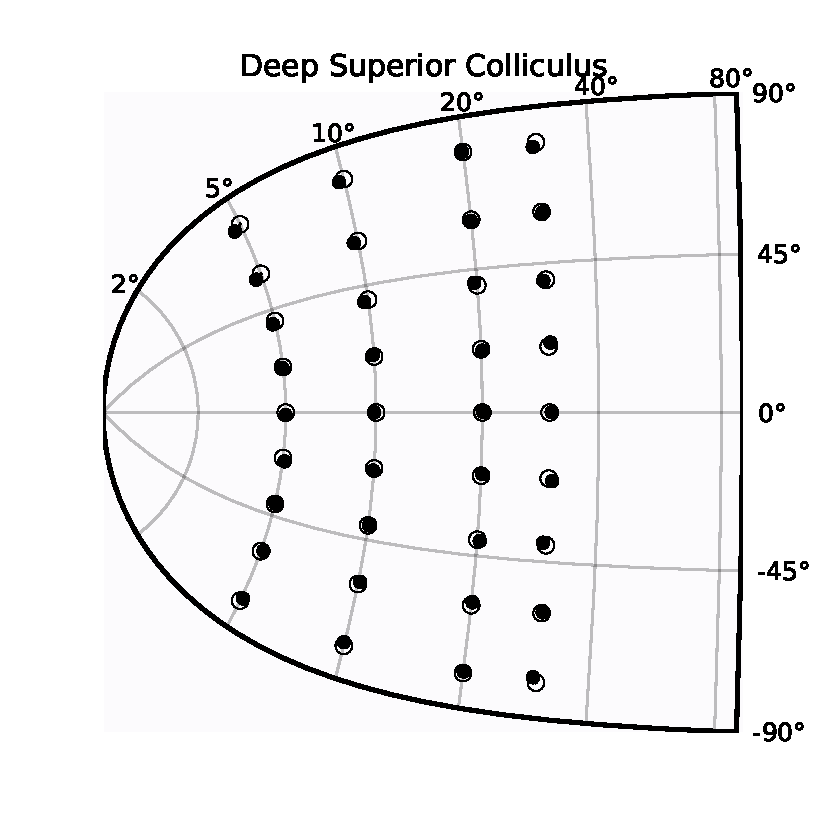
\includegraphics[width=1.0\textwidth]{Chapitres/PublicationsSample/Chapitre/figures/accuracy}
  \caption{Accuracy of the model of the superior colliculus has been measured
    using a set of retina targets that have been
    sequentially presented to the SC model. For each target and after
    convergence (difference of activity between time $t$ and time $t+dt$ is
    negligible), the center of mass of the collicular activity has been decoded
    and represented as a circle (black dots represent the
    actual projection of the target in collicular coordinates).}
  \label{fig:accuracy}
\end{figure*}

\subsubsection{Target Selection from exogenous information}

Several studies have provided data on the organization of the saccadic
path \cite{Yarbus:1967,Levy:1974,Noton:1971}. A set of
experiences on adults with normal vision showed that the attractive
value of a visual stimulus depends strongly on its distance relative
to the previous fixation point (short distances preferred). Moreover,
for several targets at the same distance, this attractive value is
greater when the eccentricity is less important (targets closer to the
fovea preferred). This result can be interpreted in the purposive
framework evoked above, associating vision and preparation for
action. In this perspective, shorter saccades are preferred and a
nearby object is more interesting than a distant object for example in
the case of hunger or danger.

Interestingly, our model displays a similar behavior and provides an
explanation that is based on the topology of the neural network
preparing the saccade. On the one hand, the spatial distribution of
collicular neurons and their receptive fields resulting from the
log-polar transformation (cortical magnification) reflect in a
qualitative way how the visual information is transformed from the
retina to the motor map of the superior colliculus. A visual stimulus
projected onto the foveal region evokes more neural activity (on the
rostral part of the collicular map) than a similar stimulus in the
peripheral region.  On the other hand, the connectivity of the DNF
model plays the role of a "winner-take-all". The profile of inhibition
ensures that the system reaches a stable state once a neighborhood is
recruited; there is always a selection at the end of the process. But
this selection made at the premotor level does not always reflect a
sensory selection: In some cases, the recruited population corresponds
to an averaging and the final target may be a position where there is
no stimulus; this depends on the profile of the lateral connections.
Figure \ref{fig:selection} reports an experiment where the model is
tested using two punctual equivalent stimuli (same aperture, intensity
and shape).  Their attractive value is estimated in V1 map.  The
cortical population activated by the stimulus at $3^\circ$ is larger
than the population activated by the stimulus at $10^\circ$. Then, the
resulting activity after computation in the deep layer of the superior
colliculus is a stable bubble in the first position. So it can be said
that the selection of the nearby stimulus emerges from the local
computation.

\begin{figure}
  \centering
    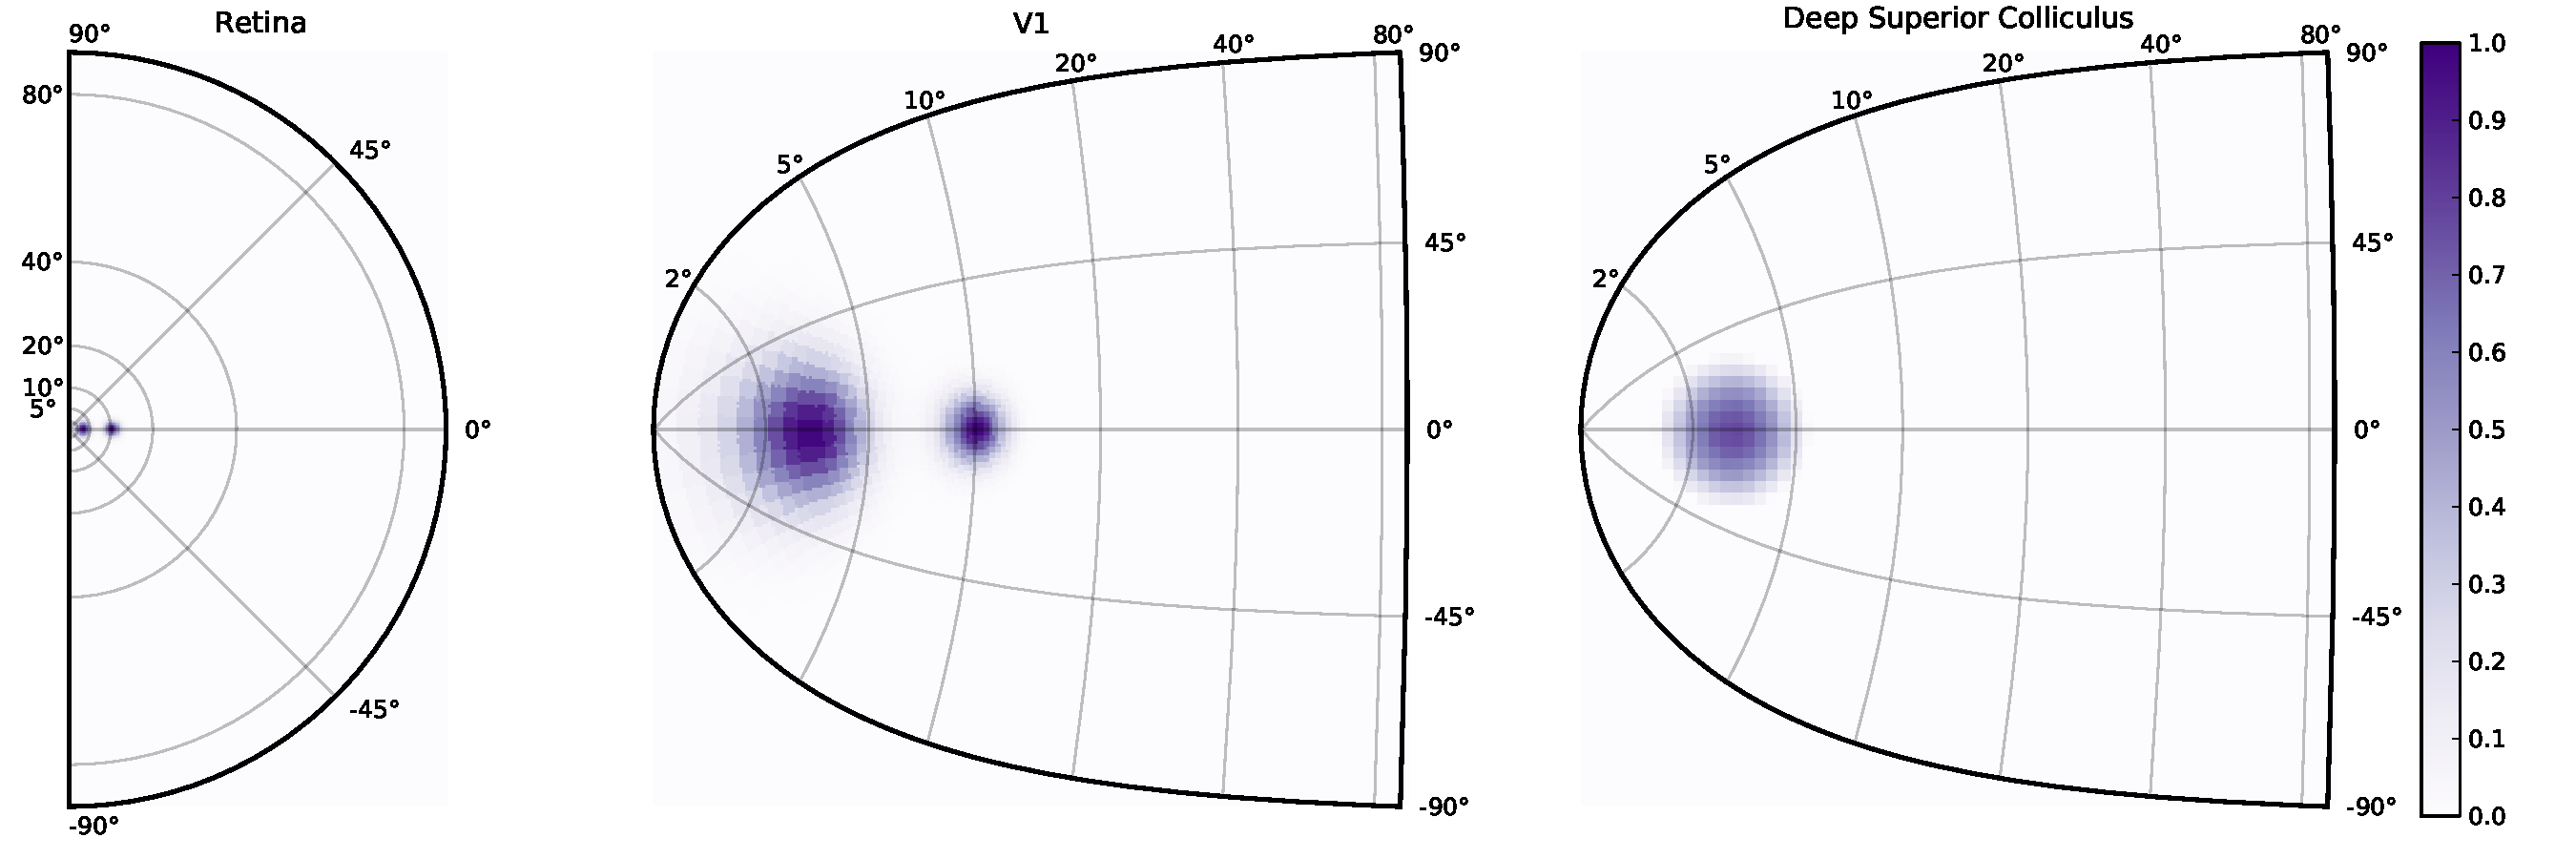
\includegraphics[width=\textwidth]{Chapitres/PublicationsSample/Chapitre/figures/selection}
  \caption{The projection of two equivalent horizontal stimuli but at different eccentricities. The stimulus nearer to the fovea is automatically selected to be the saccade target. }
  \label{fig:selection}
\end{figure}

%---------------------------------------------------------------------------
\subsubsection{Natural Images Processing}
We have also tested the model using natural images taken from a color CCD
camera. No image processing has been performed on the image but a conversion to
a gray-level representation. Figure \ref{fig:colliculus} exhibits an example
where a subpart of a computer keyboard has been shot. This allows to illustrate
the main feature of the proposed model. If one look closely at the half retina
representing the keyboard (upper left part of the figure), one can see that
several letters ({\tt O, P, L, M}) are eligible for attention focus and for
ocular saccade. However, the retinotopic projection onto the model of the V1
area reduces quite naturally this set to letters {\tt O} and {\tt L}.
\begin{figure*}
  \centering
    \includegraphics[width=1.0\textwidth]{Chapitres/PublicationsSample/Chapitre/figures/colliculus-1}\\
    \includegraphics[width=1.0\textwidth]{Chapitres/PublicationsSample/Chapitre/figures/colliculus-2}
  \caption{An image of a computer keyboard has been captured using a color
    camera (resolution $1024 \times 1280$) and transformed into a normalized
    gray level image. \textbf{Upper figure.} The right half of the image is
    presented to the half retina area which in turn feeds the V1 area where
    retinotopy is applied following equation \ref{eq:magnification}. The
    colliculus area enters a competition stage where most salient locations are
    eligible for final activation and after some iterations, the competition
    ends up onto the {\tt O} letter that is thus considered the most salient
    location of the visual scene according to its location and
    activation. \textbf{Lower figure.} A saccade has been simulated to center
    the {\tt O} letter into the center of the fovea and the colliculus now
    focuses onto a subpart of the {\tt O} letter that appears to be the newly
    most salient location of the new visual scene.}
  \label{fig:colliculus}
\end{figure*}
The model of the SC is thus confronted with a choice between these two
locations and the dynamic field theory, as it has been introduced in the
previous section, ensures that only one location remains after
competition. However it is hard to specify the exact conditions that make the
model focus on the {\tt O} instead of the {\tt L} letter in the given
example and the spatially compact shape of the {\tt O} is certainly to be taken
into account. This example also underlies the inherent difficulty in temporally
organizing ocular saccades without any top-down control. If we were to let the
model only react to its sensory input, it would certainly focus on the most
salient location without ever exploring other points of interest (from a
behavioral point of view). If the actual saccade brings into view another
salient location, the model would jump again to the new location (provided we
inhibited the foveal region to prevent the model to be stuck forever on this
single location) but in such a case, nothing would prevent the model from going
to location A then location B and then again location A, being trapped in a
cycle. Exploring the whole visual scene thus requires some kind of top down
control to be able to dynamically inhibit visited location once they have been
focused in order to favor other locations. This is out of scope of the present
article but this has been already made in a wider but less realistic model
\cite{Fix:2006}.



\subsection{Discussion}
We have introduced in this paper a model of the superior colliculus based on on
a large set of biological data. This model has been designed using a strongly
constrained modeling framework relying on a set of four computational
principles (distributed, asynchronous, numerical and adaptive) and those
properties ensure to some extent that the model does not suffer from usual
artifacts of such computational framework (presence of a central supervisor
deciding of the actual behavior). More specifically, the saccadic behavior we
exhibited through the various experiments is a true and emergent property of
local and homogeneous computations only. If we give a closer look to the
selection process that is carried out when the model is presented with two
identical stimuli (but at two different locations), we may explain the
selection of the stimuli closest to the foveal region because of the cortical
magnification. Said differently, the cortical magnification deeply influences
the network topology and consequently the saliency of any presented stimuli. If
we were to use some different magnification function, this would modify as well
the selection process. This selective behavior is thus tightly linked to the
spatial and physic implementation of the computational units. The intelligence
of the system is thus rooted in its physical instantiation (even though it is
simulated in our case).\\

However, if we now give a closer look to figure \ref{fig:magnification}, we may
realize that there is counterpart for such an automatic selection. Because the
foveal region benefits from a much higher resolution than peripheral regions,
the projections from retina to the V1 region distorts the geometrical
properties of the image. This is especially the case of straight lines that are
now projected as curved lines within the V1 region. Furthermore, the projection
of any straight line from retina to V1 is unique and does not benefit from the
same geometrical properties. How do we recognize a straight line in such
conditions ? Classical answers relying on generic neighborhood functions that
would (for example) link geometrically {\em aligned} neurons (hence mimicking
the abstract description of a geometrical line) is not possible anymore. We
thus have to change paradigm and consider new approaches like the one described
in \cite{ORegan:2001}. In this article, authors propose to reconsider vision by
integrating the sensory-motor dimension of perception. Even though a straight
line is not projected as a straight line in visual regions, there is
nonetheless a physical property that remains true independently of the physical
apparatus: if we move eyes along a straight line, there is an invariance in the
projection because this is the physical definition of a line. Such
sensori-motor behavior is a complex challenge that we are now actively
exploring in terms of the temporal organization of the saccadic behavior. In
order to achieve such active behavior, we now have to consider endogenous
inputs conveying such information as instructions, goals or motivations from
other higher-level neural structures. This lead us to consider anatomical
structure such as the basal ganglia that are known to be deeply involved with
voluntary motor control. In the end, we expect the model to achieve vision and
recognition based on motor learning that may ultimately replace {\em passive
  perception}.






